%!TEX encoding = UTF-8 Unicode
%!TEX root = ../lect-w07.tex

\Subsection{Integrerad utvecklingsmiljö (IDE)}

\begin{Slide}{Välja IDE}\SlideFontSmall
\begin{itemize}
\item En \Emph{integrerad utvecklingsmiljö} \Eng{Integrated Development Environment, IDE} innehåller \\ editor + kompilator + debugger + en massa annat\\och gör utvecklingen enklare när man lärt sig alla finesser.

\item Läs om vad en IDE kan göra i appendix I.

\pause

\item På LTH:s datorer finns två populära IDE installerade:
\begin{enumerate}\SlideFontSmall
\item \Emph{Eclipse} med plugin \Emph{ScalaIDE} förinstallerad
\begin{REPL}[numbers=none]
$ scalaide
\end{REPL}
\item \Emph{IntelliJ IDEA} (välj installera Scala-plugin när du kör första gången)
\begin{REPL}[numbers=none]
$ idea
\end{REPL}

\end{enumerate}
Läs mer om dessa i appendix D innan du väljer vilken du vill lära dig. Där står även hur du installerar dem på din egen dator. \\Flest handledare har störst vana vid Eclipse.
\end{itemize}
\end{Slide}

\begin{Slide}{Eclipse med ScalaIDE}
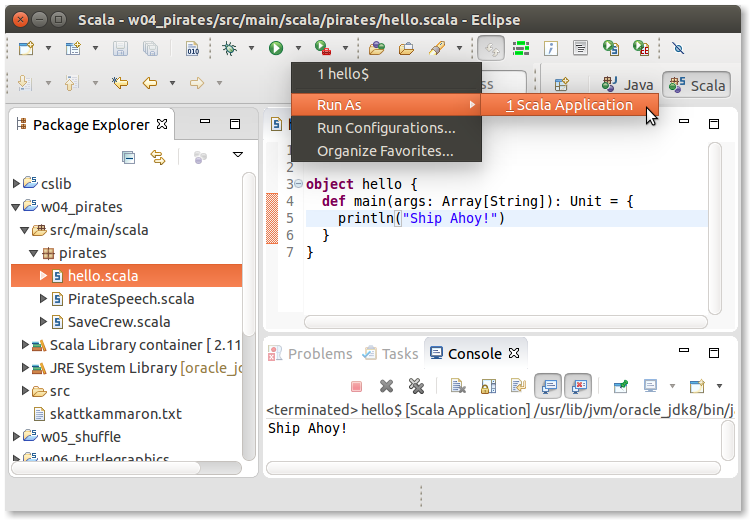
\includegraphics[width=\textwidth]{../img/eclipse/eclipse-pirates-hello.png}
\end{Slide}


\begin{Slide}{IntelliJ IDEA med Scala-plugin}
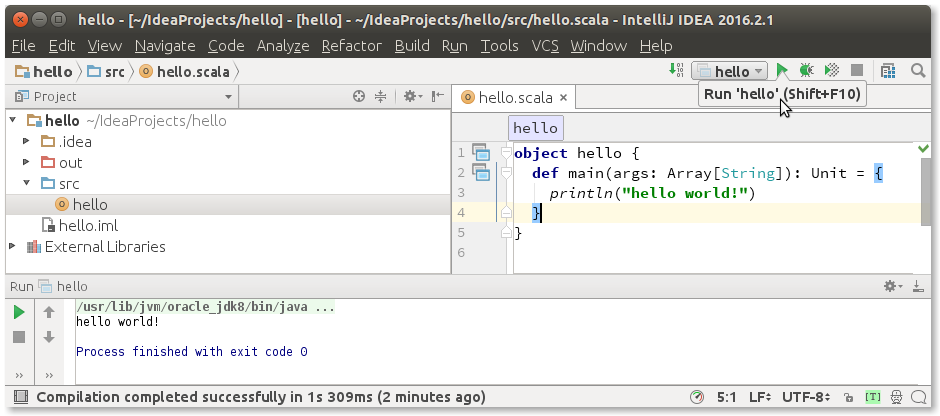
\includegraphics[width=\textwidth]{../img/intellij/idea-hello.png}
\end{Slide}

\ifkompendium\else

\begin{Slide}{Denna veckas övning: \texttt{data}}
\begin{itemize}\SlideFontTiny
%!TEX encoding = UTF-8 Unicode
%!TEX root = ../compendium2.tex

\item Kunna skapa och använda tupler, som variabelvärden, parametrar och returvärden.

\item Förstå skillnaden mellan ett objekt och en klass och kunna förklara betydelsen av begreppet instans.

\item Kunna skapa och använda attribut som medlemmar i objekt och klasser och som som klassparametrar.

\item Beskriva innebörden av och syftet med att ett attribut är privat.

\item Kunna byta ut implementationen av metoden \code{toString}.

\item Kunna skapa och använda en objektfabrik med metoden \code{apply}.

\item Kunna skapa och använda en enkel case-klass.

\item Kunna använda operatornotation och förklara relationen till punktnotation.

\item Förstå konsekvensen av uppdatering av föränderlig data i samband med multipla referenser.

\item Känna till och kunna använda några grundläggande metoder på samlingar.

\item Känna till den principiella skillnaden mellan \code{List} och \code{Vector}.

\item Kunna skapa och använda en oföränderlig mängd med klassen \code{Set}.

\item Förstå skillnaden mellan en mängd och en sekvens.

\item Kunna skapa och använda en nyckel-värde-tabell, \code{Map}.

\item Förstå likheter och skillnader mellan en \code{Map} och en \code{Vector}.

\end{itemize}
\end{Slide}

\begin{Slide}{Denna veckas laboration: \texttt{pirates}}
\begin{itemize}\SlideFontSmall
%!TEX encoding = UTF-8 Unicode
%!TEX root = ../compendium2.tex

%\item Kunna använda en integrerad utvecklingsmiljö (IDE).
%\item Kunna använda färdiga funktioner för att läsa till, och skriva från, textfil.
%\item Kunna använda enkla case-klasser.
%\item Kunna skapa och använda enkla klasser med föränderlig data.
\item Kunna skapa och använda nyckel-värde-tabeller med samlingstypen \code{Map}.
\item Kunna skapa och använda mängder med samlingstypen \code{Set}.
\item Förstå skillnaden mellan en ordnad sekvens och en mängd.
\item Förstå likheter och skillnader mellan en sekvens av par och en nyckel-värde-tabell. 
%\item Kunna skapa en ny samling från en befintlig samling.
%\item Förstå skillnaden mellan kompileringsfel och exekveringsfel.
%\item Kunna felsöka i små program med hjälp av utskrifter.
%\item Kunna felsöka i små program med hjälp av en debugger i en IDE.

\end{itemize}
\end{Slide}

\fi
